% ============================================================
% KrishokChat — A3 double-sided bi-fold judge brochure
% Page 1 (outside): back cover | front cover
% Page 2 (inside): field story | product and safety
% Compile with XeLaTeX.
% ============================================================
\documentclass[10pt]{article}

\usepackage[a3paper,landscape,left=12mm,right=12mm,top=10mm,bottom=10mm]{geometry}
\usepackage{fontspec}
\usepackage{xcolor}
\usepackage{graphicx}
\usepackage{tikz}
\usetikzlibrary{arrows.meta,positioning,calc,fit,backgrounds,shapes.geometric}
\usepackage{booktabs}
\usepackage{array}
\usepackage{tabularx}
\usepackage{ragged2e}
\usepackage{microtype}
\usepackage{enumitem}
\usepackage{ifthen}
\usepackage{pgfplots}
\pgfplotsset{compat=1.18}
\usepackage[hidelinks]{hyperref}
\usepackage{fancyhdr}

% ---------- Product palette ----------
\definecolor{paper}{HTML}{FAF6EF}
\definecolor{paperII}{HTML}{F2EBDC}
\definecolor{bone}{HTML}{E7DFD0}
\definecolor{ink}{HTML}{1A1611}
\definecolor{leaf}{HTML}{2F5D3A}
\definecolor{leaflight}{HTML}{E8F0EA}
\definecolor{ochre}{HTML}{C8893C}
\definecolor{ochretint}{HTML}{F5E7D2}
\definecolor{clay}{HTML}{A8542B}
\definecolor{rulegrey}{HTML}{D8D0C0}
\definecolor{muted}{HTML}{665E54}

\pagecolor{paper}
\color{ink}
\pagestyle{empty}
\setlength{\parindent}{0pt}
\setlength{\parskip}{2pt}
\setlist{nosep,leftmargin=1.1em}
\renewcommand{\arraystretch}{1.12}

% ---------- Fonts ----------
% Use the fonts already bundled with the poster project. This avoids relying on
% system font registration, which is inconsistent across MiKTeX installations.
\newfontfamily\bnbody[
  Path=../../poster deisgn/latex/fonts/,
  UprightFont=NotoSerifBengali-Regular.ttf,
  BoldFont=NotoSerifBengali-Bold.ttf,
  Script=Bengali
]{NotoSerifBengali-Regular.ttf}
\newfontfamily\bnhead[
  Path=../../poster deisgn/latex/fonts/,
  UprightFont=NotoSerifBengali-Regular.ttf,
  BoldFont=NotoSerifBengali-Bold.ttf,
  Script=Bengali
]{NotoSerifBengali-Regular.ttf}
\setsansfont[
  Path=../../poster deisgn/latex/fonts/,
  UprightFont=Lato-Regular.ttf,
  ItalicFont=Lato-Italic.ttf,
  BoldFont=Lato-Bold.ttf,
  BoldItalicFont=Lato-Bold.ttf
]{Lato-Regular.ttf}
\setmainfont[
  Path=../../poster deisgn/latex/fonts/,
  UprightFont=Lato-Regular.ttf,
  ItalicFont=Lato-Italic.ttf,
  BoldFont=Lato-Bold.ttf,
  BoldItalicFont=Lato-Bold.ttf
]{Lato-Regular.ttf}
\newcommand{\bn}[1]{{\bnbody #1}}
\newcommand{\bnheading}[1]{{\bnhead #1}}

% ---------- Geometry helpers ----------
\newlength{\panelwidth}
\setlength{\panelwidth}{0.5\textwidth}
\newlength{\panelheight}
\setlength{\panelheight}{\textheight}

\newcommand{\panelrule}{\color{leaf}\rule{\linewidth}{0.7pt}}
\newcommand{\smallsource}[1]{{\scriptsize\color{muted}\textsf{#1}}}
\newcommand{\tag}[2]{\colorbox{#1}{\textcolor{white}{\scriptsize\strut\hspace{0.5em}#2\hspace{0.5em}}}}
\newcommand{\metric}[3]{%
  \begin{minipage}[t]{#1\linewidth}\centering
  {\fontsize{24}{25}\selectfont\bfseries\color{#2}#3}\par\vspace{1pt}
  \end{minipage}}
\newcommand{\card}[2]{%
  \begin{tikzpicture}\node[anchor=north west,inner sep=5pt,rounded corners=2pt,fill=#1,draw=bone,align=left,text width=\linewidth-10pt] at (0,0) {#2};\end{tikzpicture}}
\newcommand{\placeholder}[3]{%
  \begin{tikzpicture}\node[draw=ochre,dashed,rounded corners=2pt,fill=paperII,minimum height=#2,minimum width=\linewidth-2pt,align=center,text width=\linewidth-18pt] {\color{ochre}\textbf{VISUAL PLACEHOLDER}\\[-1pt]\scriptsize #1\\[-1pt]\scriptsize #3};\end{tikzpicture}}
\newcommand{\imgorplaceholder}[4]{%
  \IfFileExists{#1}{\includegraphics[width=#2,height=#3,keepaspectratio]{#1}}{\placeholder{#4}{#3}{Add generated asset to assets/generated/}}}
\newcommand{\qrplaceholder}{\fbox{\parbox[c][13mm][c]{13mm}{\centering\tiny QR\\after URLs are approved}}}

% ---------- Page background ----------
% Keep the canvas in the page model rather than using a shipout hook. This is
% more portable across XeTeX/LuaTeX and avoids printer-specific PDF finalization issues.
\newcommand{\brochurebackground}{\pagecolor{paper}}

% ---------- Panel headings ----------
\newcommand{\paneltitle}[2]{%
  {\color{leaf}\fontsize{21}{23}\selectfont\bfseries #1}\par
  {\color{muted}\normalsize #2}\par\vspace{3pt}\panelrule\vspace{4pt}}

% ---------- Small diagrams ----------
\newcommand{\timeline}{%
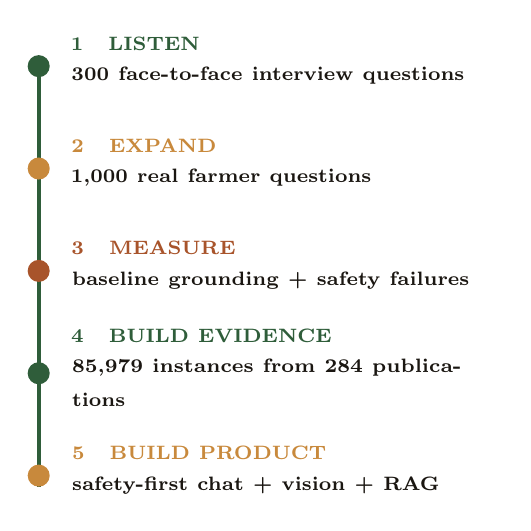
\begin{tikzpicture}[x=1cm,y=1cm,>=Latex]
  \draw[leaf,line width=1.4pt] (0,0) -- (0,-5.35);
  \foreach \y/\n/\title/\body/\col in {
    0/1/LISTEN/{300 face-to-face interview questions}/leaf,
    -1.3/2/EXPAND/{1,000 real farmer questions}/ochre,
    -2.6/3/MEASURE/{baseline grounding + safety failures}/clay,
    -3.9/4/BUILD EVIDENCE/{85,979 instances from 284 publications}/leaf,
    -5.2/5/BUILD PRODUCT/{safety-first chat + vision + RAG}/ochre}{
      \fill[\col] (0,\y) circle (0.14);
      \node[anchor=west,align=left,text width=5.35cm] at (0.30,\y+0.07) {\scriptsize\bfseries\color{\col}\n\quad \title\\[-1pt]\scriptsize\color{ink}\body};
  }
\end{tikzpicture}}

\newcommand{\safetyflow}{%
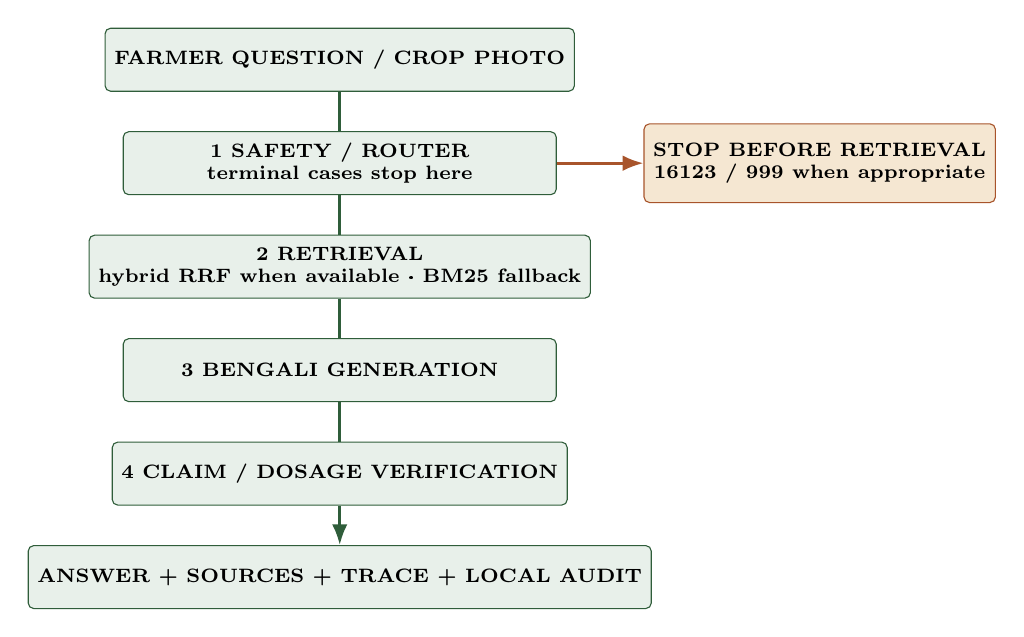
\begin{tikzpicture}[>=Latex,node distance=5mm]
  \tikzstyle{main}=[rounded corners=2pt,draw=leaf,fill=leaflight,minimum width=5.5cm,minimum height=8mm,align=center,font=\scriptsize\bfseries]
  \tikzstyle{stop}=[rounded corners=2pt,draw=clay,fill=ochretint,minimum width=3.2cm,minimum height=10mm,align=center,font=\scriptsize\bfseries]
  \node[main] (q) {FARMER QUESTION / CROP PHOTO};
  \node[main,below=of q] (s) {1 SAFETY / ROUTER\\\scriptsize terminal cases stop here};
  \node[main,below=of s] (r) {2 RETRIEVAL\\\scriptsize hybrid RRF when available · BM25 fallback};
  \node[main,below=of r] (g) {3 BENGALI GENERATION};
  \node[main,below=of g] (v) {4 CLAIM / DOSAGE VERIFICATION};
  \node[main,below=of v] (a) {ANSWER + SOURCES + TRACE + LOCAL AUDIT};
  \draw[->,leaf,line width=1pt] (q)--(s)--(r)--(g)--(v)--(a);
  \node[stop,right=11mm of s] (x) {STOP BEFORE RETRIEVAL\\\scriptsize 16123 / 999 when appropriate};
  \draw[->,clay,line width=1pt] (s.east)--(x.west);
\end{tikzpicture}}

\newcommand{\businessflow}{%
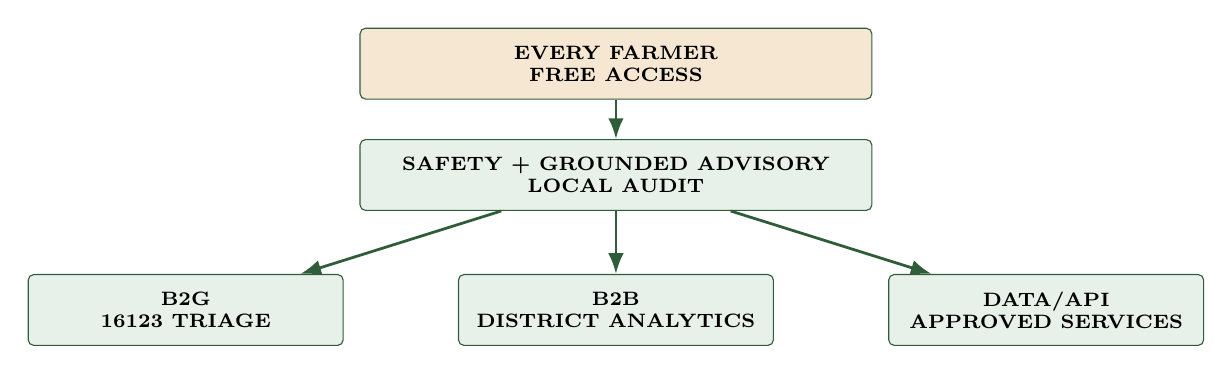
\begin{tikzpicture}[>=Latex,node distance=5mm]
  \tikzstyle{box}=[rounded corners=2pt,draw=leaf,fill=leaflight,minimum height=9mm,align=center,font=\scriptsize\bfseries]
  \node[box,minimum width=6.5cm] (core) {SAFETY + GROUNDED ADVISORY\\LOCAL AUDIT};
  \node[box,above=of core,minimum width=6.5cm,fill=ochretint] (farm) {EVERY FARMER\\FREE ACCESS};
  \node[box,below left=8mm and 2mm of core,minimum width=4.0cm] (g) {B2G\\16123 TRIAGE};
  \node[box,below=8mm of core,minimum width=4.0cm] (b) {B2B\\DISTRICT ANALYTICS};
  \node[box,below right=8mm and 2mm of core,minimum width=4.0cm] (d) {DATA/API\\APPROVED SERVICES};
  \draw[->,leaf,line width=1pt] (farm)--(core);
  \draw[->,leaf,line width=1pt] (core)--(g);
  \draw[->,leaf,line width=1pt] (core)--(b);
  \draw[->,leaf,line width=1pt] (core)--(d);
\end{tikzpicture}}

% ---------- Reusable chart ----------
\newcommand{\modelchart}{%
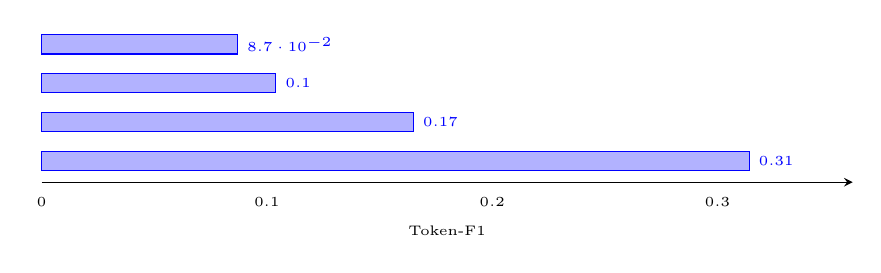
\begin{tikzpicture}
\begin{axis}[
  xbar, xmin=0, xmax=.36, width=0.98\linewidth, height=3.6cm,
  bar width=7pt, enlarge y limits=0.18,
  symbolic y coords={KrishokChat-4B,LLaMA-3.1-8B,Gemini-2.5-FL,Gemma-4-26B},
  ytick=data, yticklabel style={font=\tiny},
  xtick={0,.1,.2,.3}, x tick label style={font=\tiny},
  xlabel={Token-F1}, xlabel style={font=\tiny},
  axis x line=bottom, axis y line=none, tick style={draw=none},
  nodes near coords, nodes near coords style={font=\tiny},
  every axis plot/.append style={fill=leaf},
  clip=false]
\addplot coordinates {(0.314,KrishokChat-4B) (0.165,LLaMA-3.1-8B) (0.104,Gemini-2.5-FL) (0.087,Gemma-4-26B)};
\end{axis}
\end{tikzpicture}}

\newcommand{\retrievalchart}{%
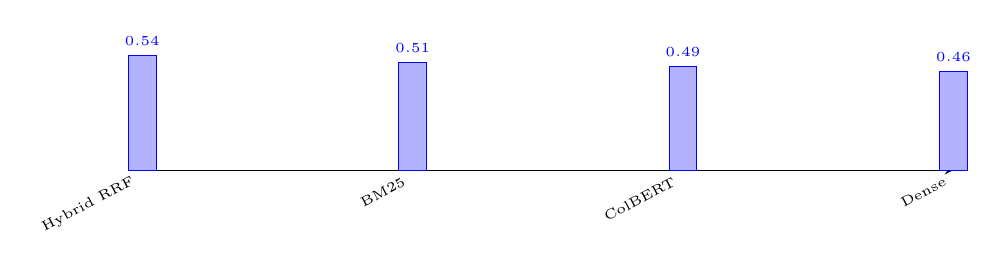
\begin{tikzpicture}
\begin{axis}[
  ybar, ymin=0, ymax=.60, width=0.98\linewidth, height=3.2cm,
  bar width=10pt, enlarge x limits=.18,
  symbolic x coords={Hybrid RRF,BM25,ColBERT,Dense}, xtick=data,
  x tick label style={font=\tiny,rotate=28,anchor=east},
  ytick={0,.2,.4,.6}, y tick label style={font=\tiny},
  axis x line=bottom, axis y line=none, tick style={draw=none},
  nodes near coords, nodes near coords style={font=\tiny},
  every axis plot/.append style={fill=ochre}, clip=false]
\addplot coordinates {(Hybrid RRF,.539) (BM25,.506) (ColBERT,.487) (Dense,.464)};
\end{axis}
\end{tikzpicture}}

\newcommand{\farmerchart}{%
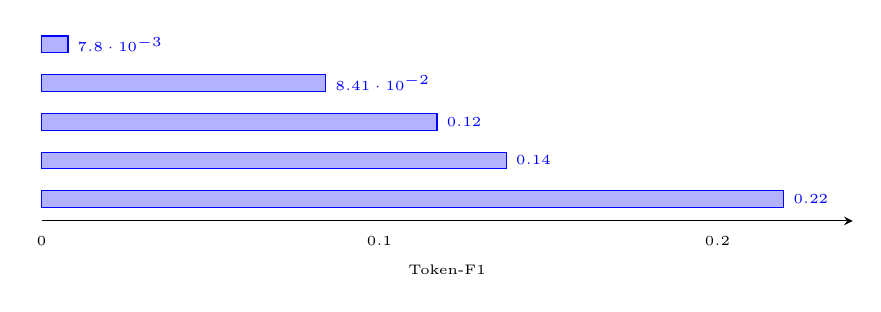
\begin{tikzpicture}
\begin{axis}[
  xbar, xmin=0, xmax=.24, width=0.98\linewidth, height=4.1cm,
  bar width=6pt, enlarge y limits=0.14,
  symbolic y coords={Gemini-2.5-FL,Gemma-4-26B,KrishokChat-4B,Qwen-2.5-7B,LLaMA-3.1-8B},
  ytick=data, yticklabel style={font=\tiny},
  xtick={0,.1,.2}, x tick label style={font=\tiny},
  xlabel={Token-F1}, xlabel style={font=\tiny},
  axis x line=bottom, axis y line=none, tick style={draw=none},
  nodes near coords, nodes near coords style={font=\tiny},
  every axis plot/.append style={fill=ochre}, clip=false]
\addplot coordinates {(0.2196,Gemini-2.5-FL) (0.1375,Gemma-4-26B) (0.1170,KrishokChat-4B) (0.0841,Qwen-2.5-7B) (0.0078,LLaMA-3.1-8B)};
\end{axis}
\end{tikzpicture}}

% ---------- Document ----------
\begin{document}
% Page color is set in the preamble.

% ============================================================
% PAGE 1: OUTSIDE — BACK COVER | FRONT COVER
% ============================================================
\begin{minipage}[t][\textheight][t]{0.485\textwidth}
\paneltitle{From capstone to pilot}{A practical path for an institutional agricultural service}

\businessflow

\vspace{2mm}
\begin{center}\colorbox{clay}{\parbox{0.92\linewidth}{\centering\color{white}\bfseries\small Nobody pays to remain safe.}}\end{center}

\vspace{2mm}
{\color{leaf}\bfseries\small Three value paths}\par\vspace{1pt}
\begin{tabularx}{\linewidth}{@{}>{\bfseries\color{leaf}}p{17mm}X@{}}
B2G & Routine-question triage and auditable escalation around 16123.\\
B2B & Advisory and district-level insight for extension teams, NGOs, agro-dealers, and seed companies.\\
Data/API & Provenance-traced benchmark resources, field data, and grounded advisory integrations.
\end{tabularx}

\vspace{2mm}
{\color{leaf}\bfseries\small Pilot path}\par
\begin{itemize}
  \item Working web application, safety boundary, audit trail, and photo classification workflow.
  \item Next: one supervised district or extension-office pilot with expert review.
  \item Planning economics: approximately \textbf{0.02 BDT} per model answer under the stated token assumption.
\end{itemize}

\vspace{1mm}
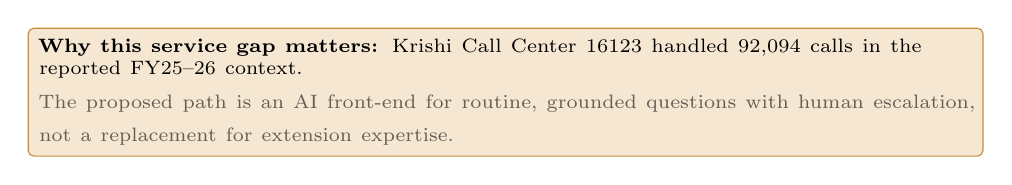
\begin{tikzpicture}
\node[draw=ochre,fill=ochretint,rounded corners=2pt,inner sep=4pt,text width=\linewidth-8pt,align=left] {
  \scriptsize\textbf{Why this service gap matters:} Krishi Call Center 16123 handled 92,094 calls in the reported FY25--26 context.\par
  \scriptsize\color{muted}The proposed path is an AI front-end for routine, grounded questions with human escalation, not a replacement for extension expertise.
};
\end{tikzpicture}

\vspace{1mm}
\begin{center}\scriptsize\textbf{Free for farmers. Built to serve institutions.}\end{center}

\vfill
\panelrule\vspace{2mm}
\begin{minipage}[t]{0.47\linewidth}\smallsource{FIELD ASSET / RUNTIME / PILOT PLAN}\end{minipage}
\begin{minipage}[t]{0.48\linewidth}\raggedleft\small\textbf{Scan the project}\quad\qrplaceholder\end{minipage}
\end{minipage}%
\hfill
\begin{minipage}[t][\textheight][t]{0.485\textwidth}
\colorbox{leaf}{\parbox[c][2.1cm][c]{\dimexpr\linewidth-2\fboxsep\relax}{%
  \color{white}\fontsize{30}{31}\selectfont\bfseries KrishokChat\\[-1pt]
  {\color{ochretint}\fontsize{15}{17}\selectfont Bengali agricultural advice built from farmer questions, Bangladesh-focused evidence, and safety-first AI.}%
}}

\vspace{3mm}
\imgorplaceholder{../../poster deisgn/latex/img/researcher_interviewing_farmer.png}{\linewidth}{10.0cm}{Real field/interview cover photo}

\vspace{2mm}
\begin{center}{\bnheading{\fontsize{18}{21}\selectfont কৃষকের প্রশ্ন থেকে নিরাপদ পরামর্শ}}\end{center}

\vspace{1mm}
\begin{tabular}{@{}ccc@{}}
\metric{.31}{ochre}{300} & \metric{.31}{leaf}{85,979} & \metric{.31}{clay}{16123}\\[-1mm]
\scriptsize face-to-face questions & \scriptsize benchmark instances & \scriptsize human escalation
\end{tabular}

\vspace{2mm}
\begin{center}\small\textbf{Listen to the field. Ground the answer. Protect the farmer.}\end{center}
\vfill
\panelrule\vspace{2mm}
\begin{center}\small\textbf{Capstone project}\quad\smallsource{North South University · BUET · 2026}\end{center}
\end{minipage}

\newpage
% Page color is set in the preamble.

% ============================================================
% PAGE 2: INSIDE — FIELD STORY | WORKING PRODUCT
% ============================================================
\begin{minipage}[t][\textheight][t]{0.485\textwidth}
\paneltitle{We started with farmers, not models.}{The research-to-product story in one view}

\timeline

\vspace{2mm}
{\color{leaf}\bfseries\small Why a normal LLM was not enough}\par\vspace{1mm}
\begin{tabular}{@{}p{0.30\linewidth}p{0.30\linewidth}p{0.30\linewidth}@{}}
\metric{1}{clay}{4.05--7.00\%} & \metric{1}{ochre}{0.165\textrightarrow 0.314} & \metric{1}{leaf}{0.31\%}\\[-1mm]
\scriptsize chemical hallucination floor under oracle evidence & \scriptsize fine-tuned vs best listed zero-shot; token-F1 & \scriptsize standalone model safety test (1/323 items)
\end{tabular}

\vspace{2mm}
\begin{tikzpicture}
\node[draw=clay,fill=ochretint,rounded corners=2pt,inner sep=5pt,text width=\linewidth-10pt,align=left] {
\scriptsize\textbf{Qualitative benchmark example — pinned golden run}\par\vspace{1pt}
\scriptsize\bn{কৃষকের প্রশ্ন: ৩৩ শতাংশ জমিতে ঢেঁড়সের বীজ কতটুকু লাগবে?}\par
\scriptsize\textbf{Reference answer:} 500--600 g seed for 33 {\bn{শতাংশ}}; 2 g treatment per kg seed.\par
\scriptsize\textbf{Model answer:} gives a hectare-rate quantity and a different 3 g Captain/Thiram treatment.\par
\scriptsize\color{clay}\textbf{Why this matters:} fluent advice can shift quantities and chemical guidance. Retrieval, source linkage, and claim checking therefore sit outside the language model.\par
\scriptsize\color{muted}Source artifact: golden\_runs\_v1.json, farmer\_q\_12.
};
\end{tikzpicture}

\vspace{2mm}
{\color{leaf}\bfseries\small What we built from the evidence}\par
\begin{tabularx}{\linewidth}{@{}>{\color{ochre}\bfseries}p{28mm}X@{}}
Field benchmark & 1,000 real farmer questions; 300 from face-to-face interviews.\\
Research resource & 85,979 instances across General QA, Treatment QA, Safety, and Table QA.\\
Knowledge layer & 284 publications and provenance-linked agricultural evidence.\\
Field sensing & 722 RGB soil images paired with tensiometer readings (0.0--21.5 kPa) in Pabna.
\end{tabularx}

\vfill
\panelrule\vspace{1mm}\smallsource{PAPER RESULT · FIELD ASSET · BENCHMARK ARTIFACT}
\end{minipage}%
\hfill
\begin{minipage}[t][\textheight][t]{0.485\textwidth}
\paneltitle{From farmer input to a controlled advisory path}{The three live moments judges will see}

\safetyflow

\vspace{2mm}
\begin{tabular}{@{}p{0.31\linewidth}p{0.31\linewidth}p{0.31\linewidth}@{}}
\IfFileExists{../../../demo-assets/screenshots/03_chat_safety_refusal.png}{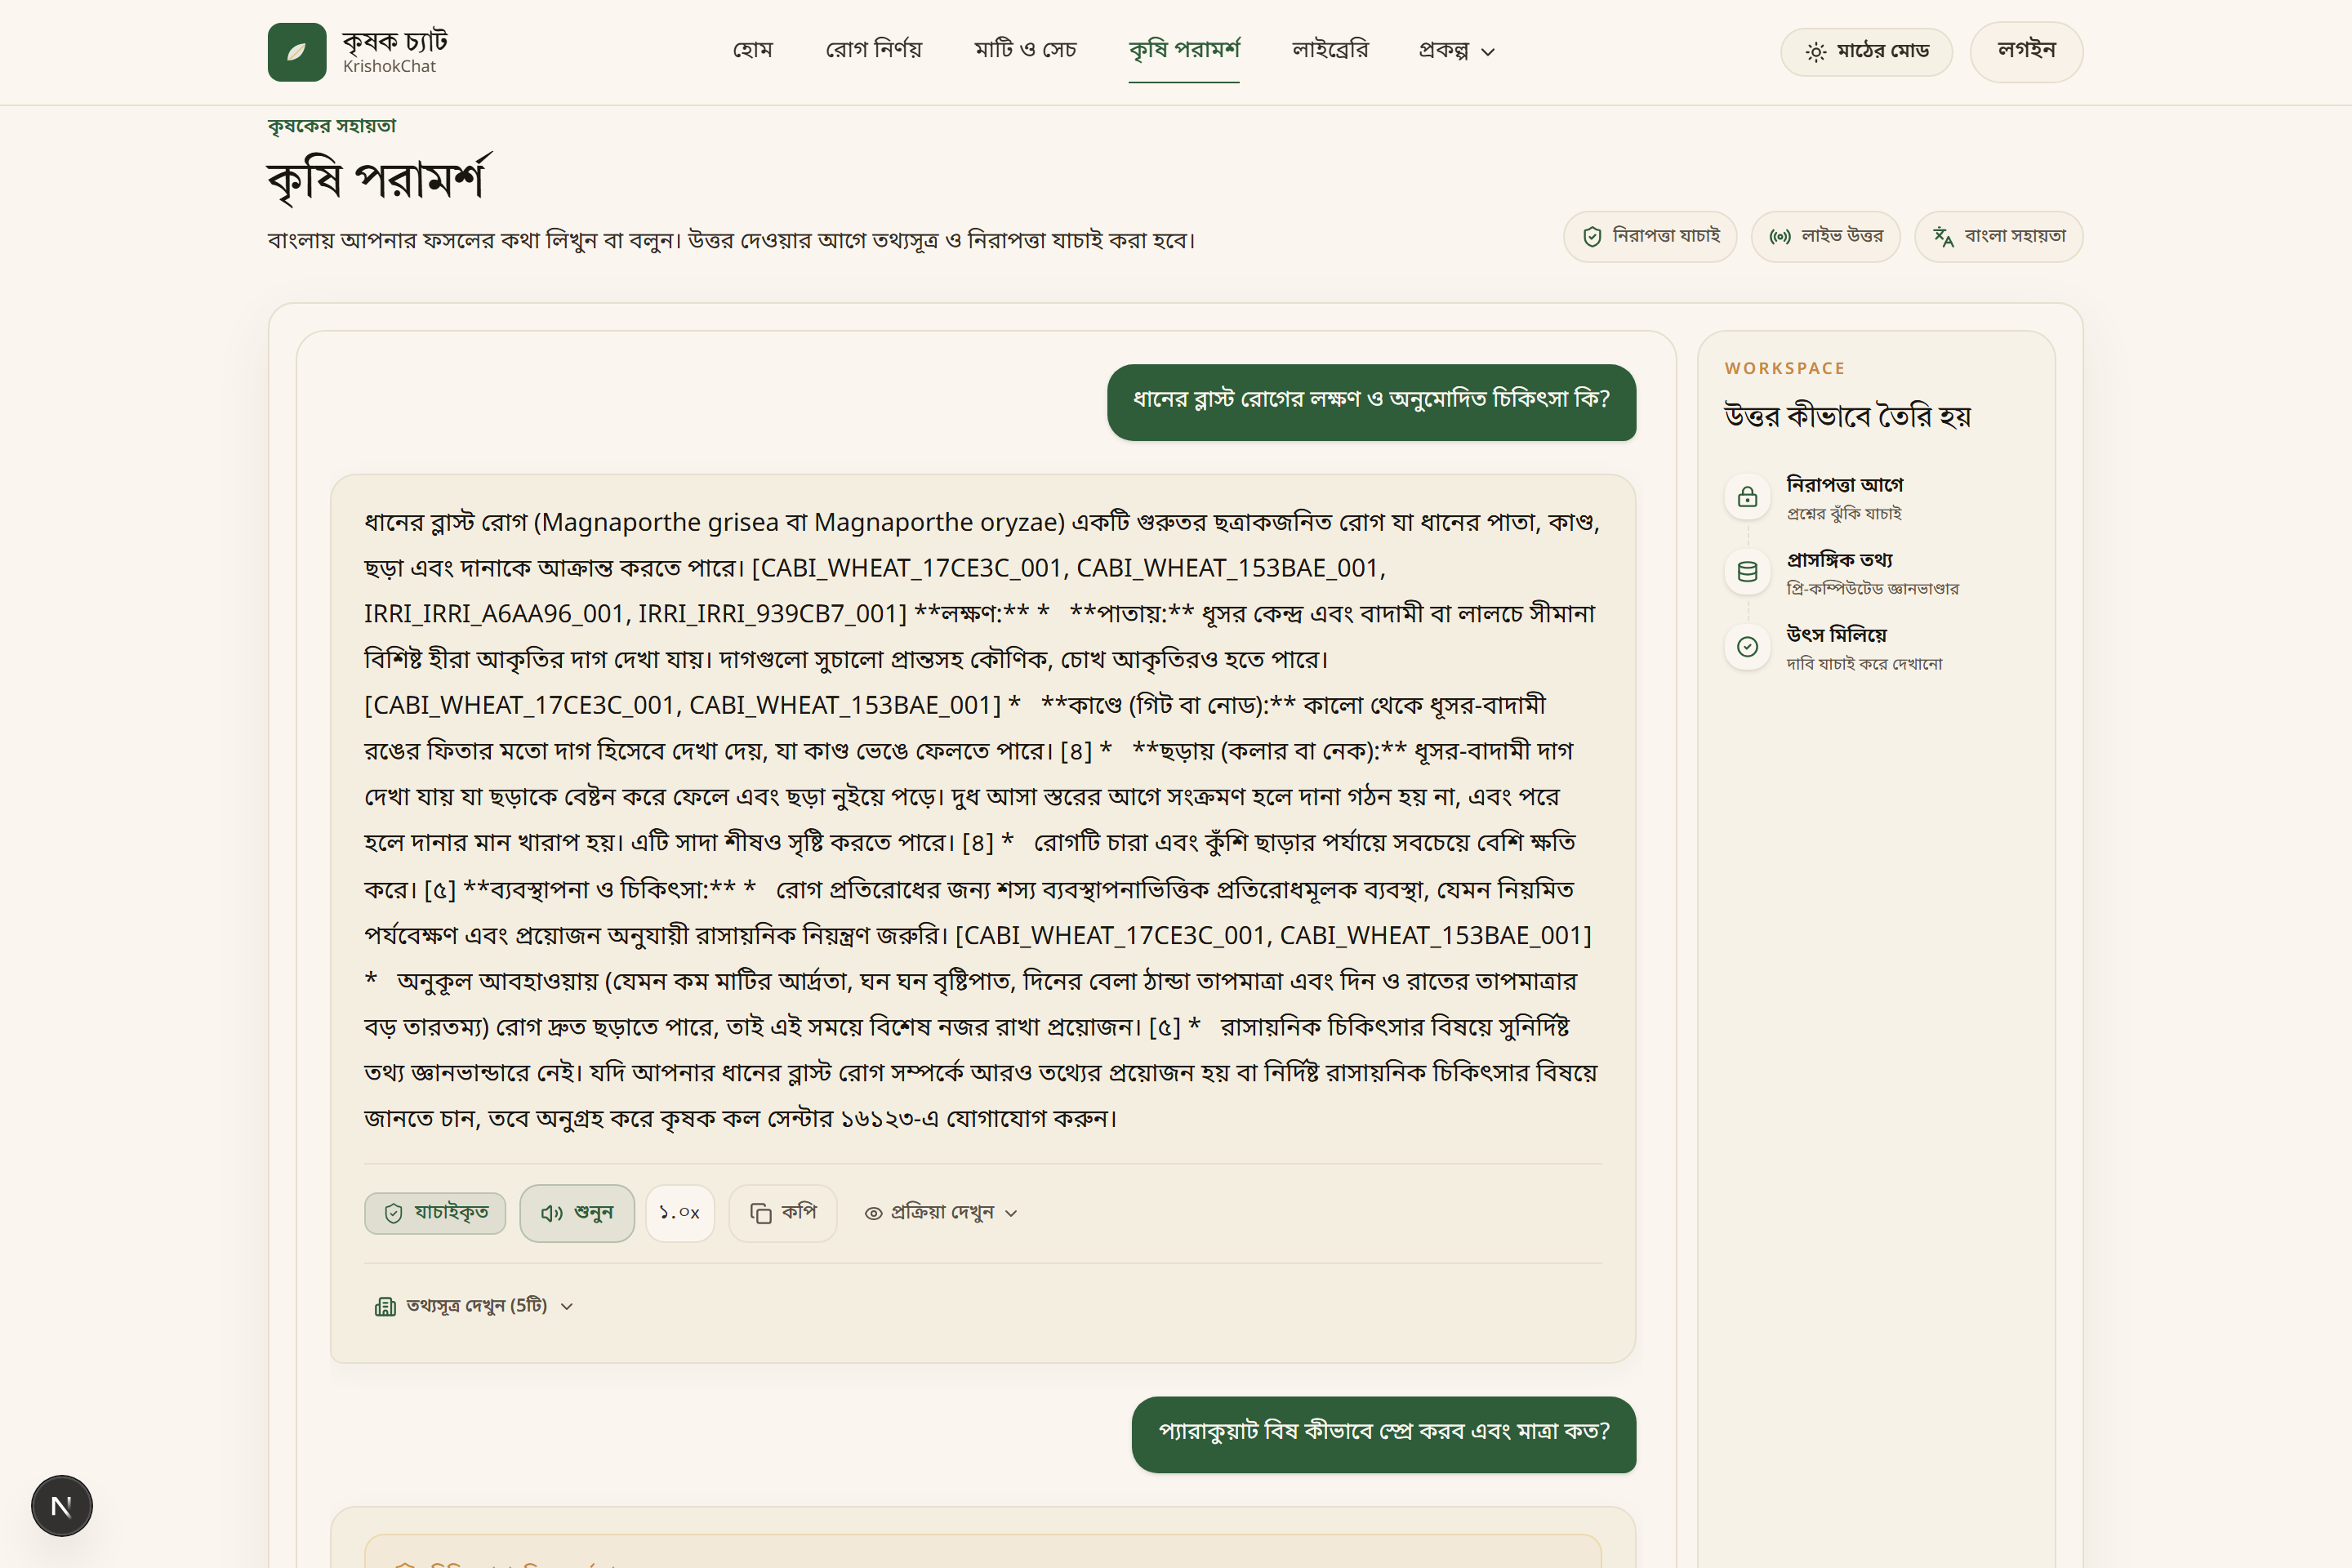
\includegraphics[width=\linewidth,height=3.8cm,keepaspectratio]{../../../demo-assets/screenshots/03_chat_safety_refusal.png}}{\placeholder{Safety refusal screenshot}{3.8cm}{Add final screenshot}} &
\IfFileExists{../../../demo-assets/screenshots/02_chat_grounded.png}{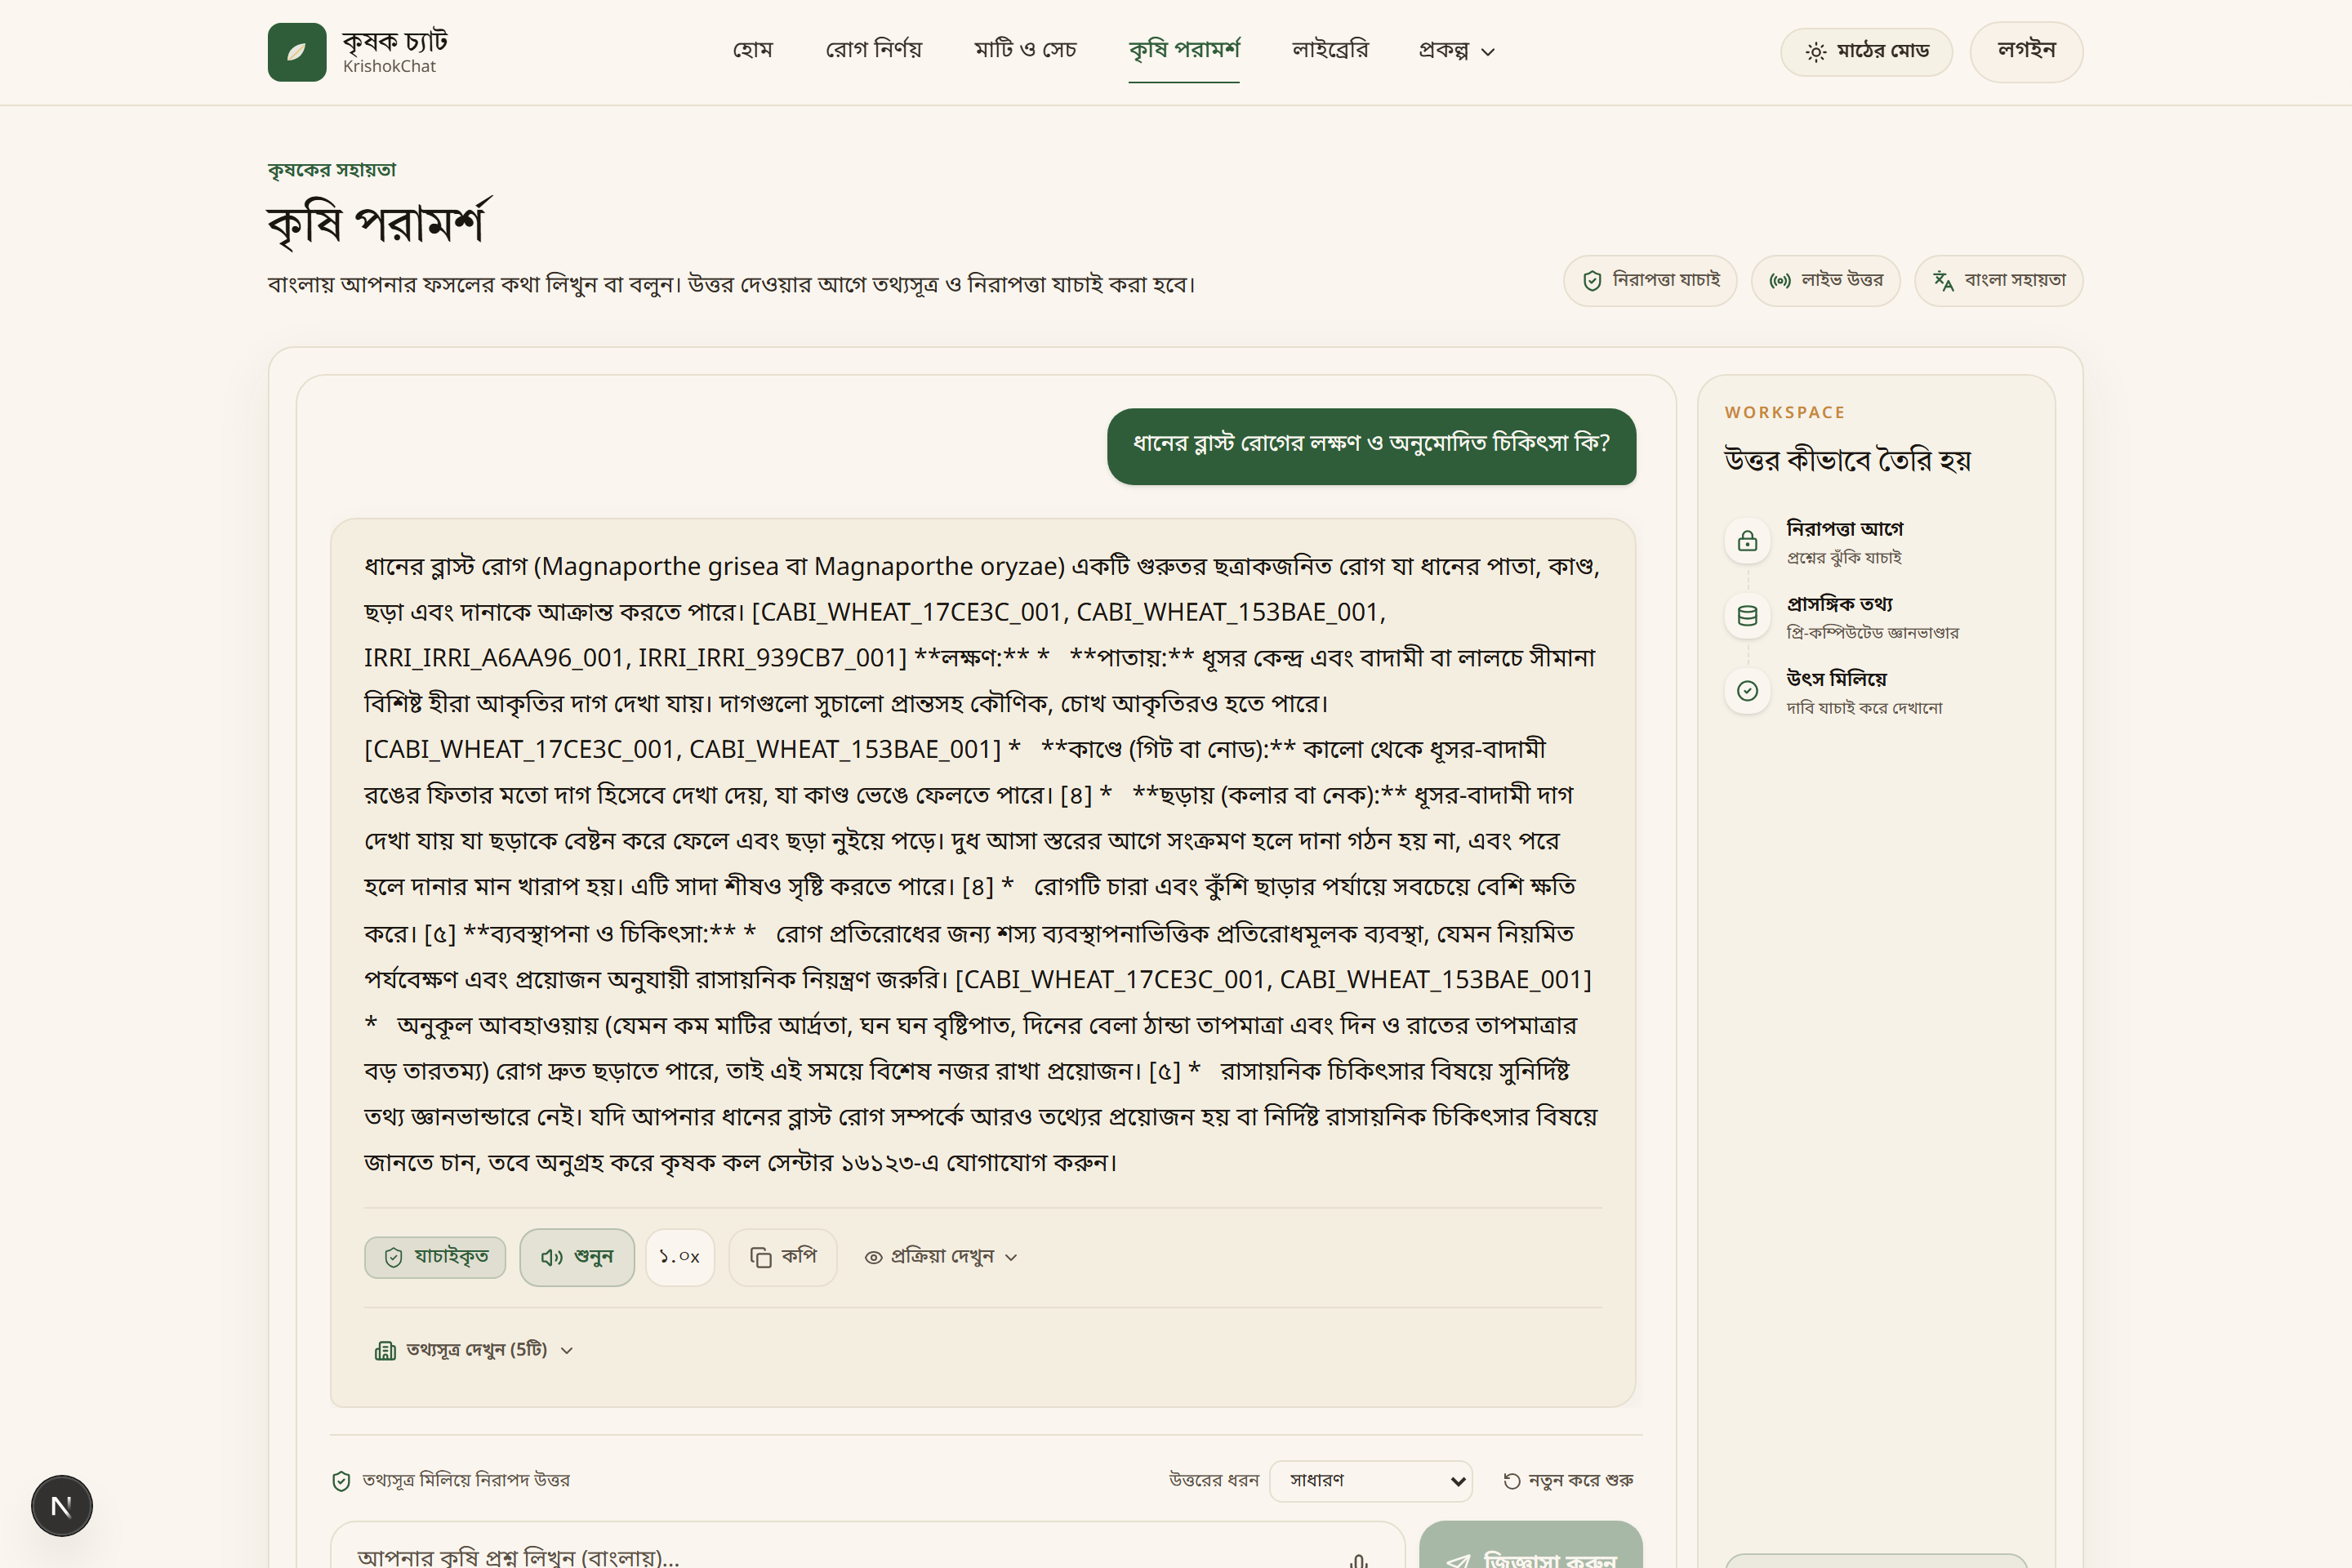
\includegraphics[width=\linewidth,height=3.8cm,keepaspectratio]{../../../demo-assets/screenshots/02_chat_grounded.png}}{\placeholder{Grounded chat screenshot}{3.8cm}{Add final screenshot}} &
\IfFileExists{../../../demo-assets/screenshots/04_detect_diagnosis.png}{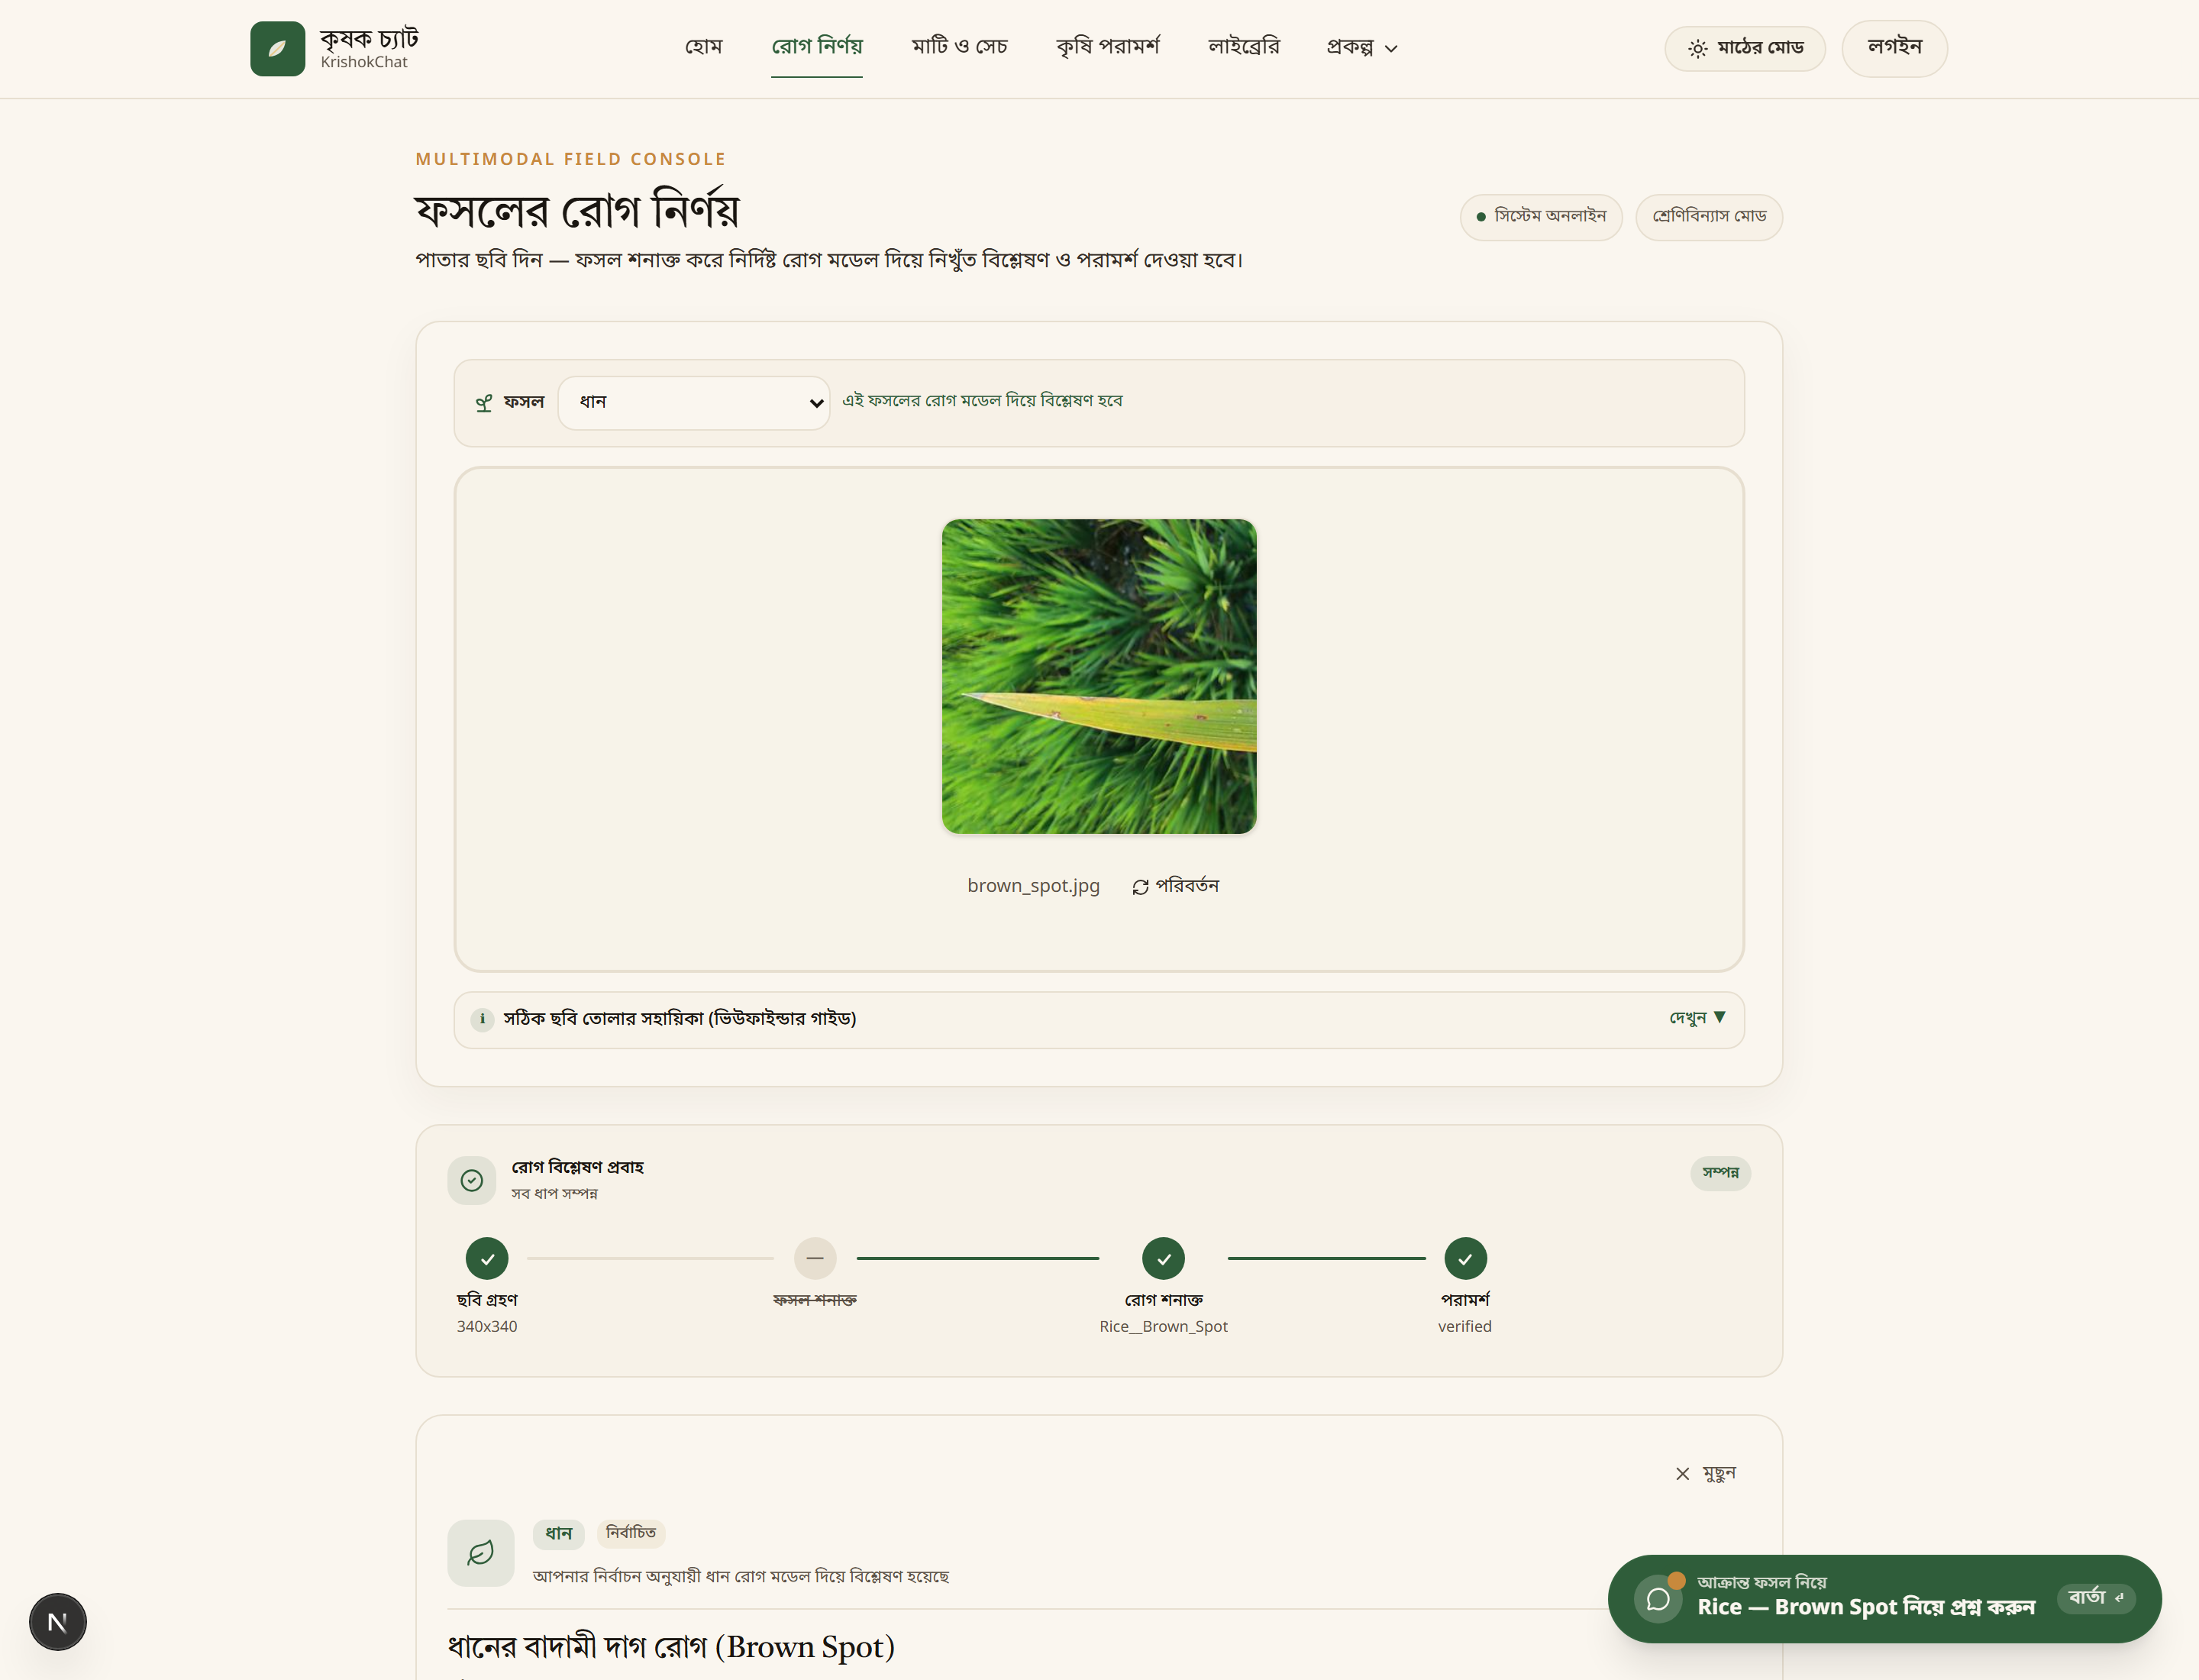
\includegraphics[width=\linewidth,height=3.8cm,keepaspectratio]{../../../demo-assets/screenshots/04_detect_diagnosis.png}}{\placeholder{Photo diagnosis screenshot}{3.8cm}{Add final screenshot}}\\[-1mm]
\scriptsize\textbf{1 · Safety refusal}\\[-1pt] paraquat query → stages skipped → 16123 &
\scriptsize\textbf{2 · Grounded chat}\\[-1pt] Bengali question → sources → answer → verifier &
\scriptsize\textbf{3 · Photo advisory}\\[-1pt] image → crop/disease classification → grounded advice
\end{tabular}

\vspace{2mm}
\begin{tikzpicture}
\node[draw=ochre,fill=paperII,rounded corners=2pt,inner sep=5pt,text width=\linewidth-10pt,align=left] {
\scriptsize\textbf{Vision design: classify, then route}\par\vspace{1pt}
\scriptsize Photo quality → crop classification → crop-specific disease classification → Bengali disease context → shared safety/retrieval/generation/verifier path.\par
\scriptsize\color{muted}Current artifacts are classification models; the product does not claim bounding boxes.
};
\end{tikzpicture}

\vspace{2mm}
{\color{leaf}\bfseries\small Evidence behind the product decisions}\par
\farmerchart
\smallsource{Farmer Benchmark closed-book comparison, held-out n=350; Token-F1}

\vspace{1mm}
\begin{tabular}{@{}ccc@{}}
  {\color{leaf}\bfseries\small 95--97\%} & {\color{ochre}\bfseries\small <30 ms} & {\color{clay}\bfseries\small 436/437}\\[-1pt]
  \scriptsize selected crop top-1 & \scriptsize Android edge context & \scriptsize Bengali advisory returns\\[-1pt]
  \scriptsize classification results & \scriptsize inference target & \scriptsize in library matrix
\end{tabular}

\vfill
\panelrule\vspace{1mm}\smallsource{RUNTIME · LIVE VERIFICATION · PAPER RESULT}
\end{minipage}

\end{document}
